\PassOptionsToPackage{unicode=true}{hyperref} % options for packages loaded elsewhere
\PassOptionsToPackage{hyphens}{url}
%
\documentclass[]{article}
\usepackage{lmodern}
\usepackage{amssymb,amsmath}
\usepackage{ifxetex,ifluatex}
\usepackage{fixltx2e} % provides \textsubscript
\ifnum 0\ifxetex 1\fi\ifluatex 1\fi=0 % if pdftex
  \usepackage[T1]{fontenc}
  \usepackage[utf8]{inputenc}
  \usepackage{textcomp} % provides euro and other symbols
\else % if luatex or xelatex
  \usepackage{unicode-math}
  \defaultfontfeatures{Ligatures=TeX,Scale=MatchLowercase}
\fi
% use upquote if available, for straight quotes in verbatim environments
\IfFileExists{upquote.sty}{\usepackage{upquote}}{}
% use microtype if available
\IfFileExists{microtype.sty}{%
\usepackage[]{microtype}
\UseMicrotypeSet[protrusion]{basicmath} % disable protrusion for tt fonts
}{}
\IfFileExists{parskip.sty}{%
\usepackage{parskip}
}{% else
\setlength{\parindent}{0pt}
\setlength{\parskip}{6pt plus 2pt minus 1pt}
}
\usepackage{hyperref}
\hypersetup{
            pdftitle={SDS 291 - Multiple Regression - Day 02},
            pdfborder={0 0 0},
            breaklinks=true}
\urlstyle{same}  % don't use monospace font for urls
\usepackage[margin=1in]{geometry}
\usepackage{graphicx,grffile}
\makeatletter
\def\maxwidth{\ifdim\Gin@nat@width>\linewidth\linewidth\else\Gin@nat@width\fi}
\def\maxheight{\ifdim\Gin@nat@height>\textheight\textheight\else\Gin@nat@height\fi}
\makeatother
% Scale images if necessary, so that they will not overflow the page
% margins by default, and it is still possible to overwrite the defaults
% using explicit options in \includegraphics[width, height, ...]{}
\setkeys{Gin}{width=\maxwidth,height=\maxheight,keepaspectratio}
\setlength{\emergencystretch}{3em}  % prevent overfull lines
\providecommand{\tightlist}{%
  \setlength{\itemsep}{0pt}\setlength{\parskip}{0pt}}
\setcounter{secnumdepth}{0}
% Redefines (sub)paragraphs to behave more like sections
\ifx\paragraph\undefined\else
\let\oldparagraph\paragraph
\renewcommand{\paragraph}[1]{\oldparagraph{#1}\mbox{}}
\fi
\ifx\subparagraph\undefined\else
\let\oldsubparagraph\subparagraph
\renewcommand{\subparagraph}[1]{\oldsubparagraph{#1}\mbox{}}
\fi

% set default figure placement to htbp
\makeatletter
\def\fps@figure{htbp}
\makeatother


\title{SDS 291 - Multiple Regression - Day 02}
\author{}
\date{\vspace{-2.5em}January 29, 2020}

\begin{document}
\maketitle

Biologists know that the leaves on plants tend to get smaller as
temperatires rise. The dataset \texttt{LeafWidth} has fata on samples of
leaves from the species \emph{Dodonaea viscosa} subsp,
\emph{angustissima}, which have been collected in a certain region of
South Australia for man years.

The variable \texttt{Width} is the average width, in mm, of leaves,
taken at their widest points, that wer collected in a given year.

\hypertarget{scatterplot-of-leaf-width-mm-and-year}{%
\subsection{1. Scatterplot of Leaf Width (mm) and
Year}\label{scatterplot-of-leaf-width-mm-and-year}}

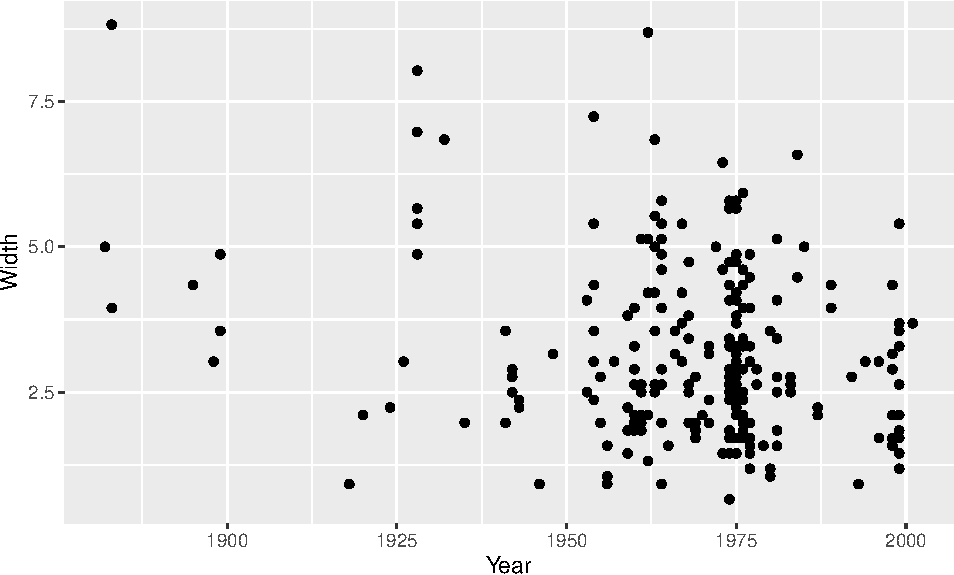
\includegraphics{02_Activity_AfterClass_files/figure-latex/scatter-1.pdf}

\hypertarget{describe-the-scatterplot-in-words.}{%
\subsubsection{Describe the scatterplot in
words.}\label{describe-the-scatterplot-in-words.}}

There is a negative, moderately weak, shallow magnitude, linear pattern
with a few unusual observations, especially in the older years.

\hypertarget{find-the-least-squares-regression-line-for-predicting-leaf-width-based-on-year}{%
\subsection{2. Find the least squares regression line for predicting
leaf width based on
year}\label{find-the-least-squares-regression-line-for-predicting-leaf-width-based-on-year}}

\begin{verbatim}
## 
## Call:
## lm(formula = Width ~ Year, data = LeafWidth)
## 
## Residuals:
##     Min      1Q  Median      3Q     Max 
## -3.1214 -1.1253 -0.3136  0.9320  5.4144 
## 
## Coefficients:
##              Estimate Std. Error t value Pr(>|t|)    
## (Intercept) 37.723091   8.574977   4.399 1.61e-05 ***
## Year        -0.017560   0.004358  -4.029 7.43e-05 ***
## ---
## Signif. codes:  0 '***' 0.001 '**' 0.01 '*' 0.05 '.' 0.1 ' ' 1
## 
## Residual standard error: 1.424 on 250 degrees of freedom
## Multiple R-squared:  0.06098,    Adjusted R-squared:  0.05723 
## F-statistic: 16.24 on 1 and 250 DF,  p-value: 7.425e-05
\end{verbatim}

\hypertarget{write-the-fitted-regression-model}{%
\subsubsection{Write the fitted regression
model}\label{write-the-fitted-regression-model}}

The fitted regression model is \(Y = \hat{\beta}_0 + \hat{\beta}_1Year\)
or \(Y = 37.723 - 0.018(Year)\)

\hypertarget{interpret-the-value-of-the-slope-for-the-fitted-model-in-the-context-of-this-setting.}{%
\subsubsection{Interpret the value of the slope for the fitted model in
the context of this
setting.}\label{interpret-the-value-of-the-slope-for-the-fitted-model-in-the-context-of-this-setting.}}

Over time, leaf widths got smaller by, on average, -0.018mm each year.

\hypertarget{assessing-the-model}{%
\subsection{3. Assessing the model}\label{assessing-the-model}}

\hypertarget{what-leaf-width-would-the-fitted-model-predict-a-leaf-in-1994-would-have}{%
\subsection{What leaf width would the fitted model predict a leaf in
1994 would
have?}\label{what-leaf-width-would-the-fitted-model-predict-a-leaf-in-1994-would-have}}

\[ \hat{y} = 37.723 + (-0.018 \cdot 1994) \]

\[ \hat{y} = 37.723 -35.01464 \]

\[ \hat{y} = 2.70836 \]

This model predicted that a leaf in 1994 would have a width of 2.71 mm.

\hypertarget{find-the-residual}{%
\subsection{Find the residual}\label{find-the-residual}}

\begin{verbatim}
##      Width   Length  LWRatio    Area Year
## 1 3.026316 61.44737 20.30435 119.027 1994
\end{verbatim}

We see from above that the actual width (y) was 3.026316.

For a given observation (\(_i\)), the residual is:

\[ Residual_i = y_i - \hat{y}_i \]

Thus the residual for this particular year was 3.026316-2.70836 =
0.317956.

Since this is a positive residual, we know that the model
\emph{underestimated} the width by 0.32 mm; that the actual value was
larger than what the model predicted it would have been.

\hypertarget{visualize-the-model}{%
\subsection{4. Visualize the model}\label{visualize-the-model}}

\hypertarget{make-a-scatterplot-that-includes-the-regression-line}{%
\subsubsection{Make a scatterplot that includes the regression
line}\label{make-a-scatterplot-that-includes-the-regression-line}}

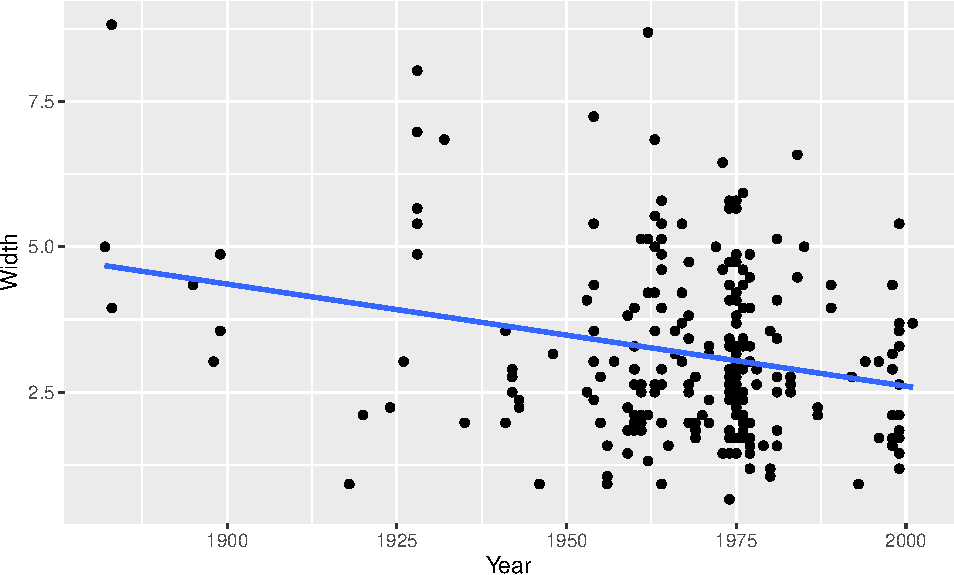
\includegraphics{02_Activity_AfterClass_files/figure-latex/unnamed-chunk-1-1.pdf}

\hypertarget{make-a-histogram-of-the-residuals}{%
\subsection{Make a histogram of the
residuals}\label{make-a-histogram-of-the-residuals}}

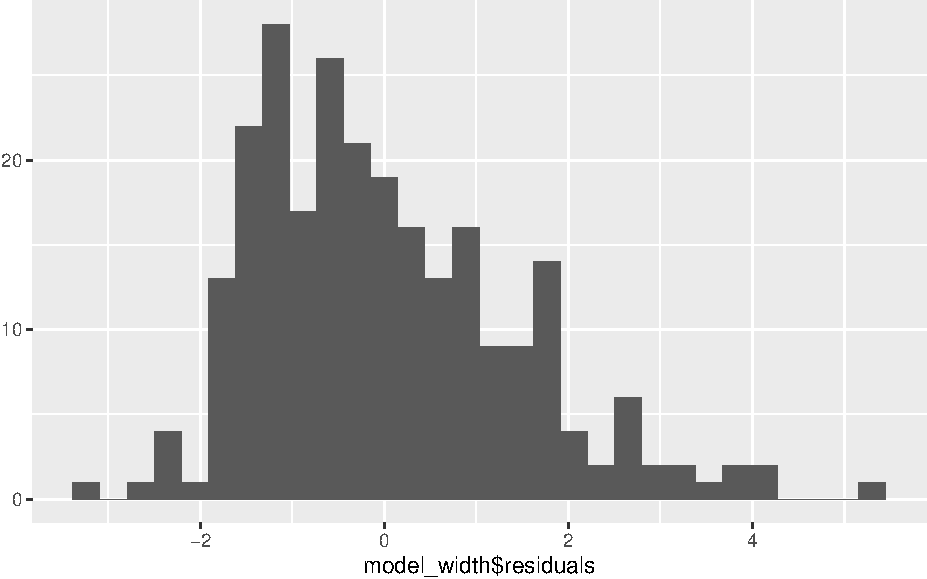
\includegraphics{02_Activity_AfterClass_files/figure-latex/unnamed-chunk-2-1.pdf}

Here, we see that the residuals are not normally distributed, that the
mean value may be 0, but that there are large positive residuals that
create a skewed distribution of the residuals. We can see visually from
the scatterplot with the regression model above that there are many more
points substantially above the line -- especially before 1950 or so.

\hypertarget{make-a-probability-plot-and-residual-fitted-plot}{%
\subsection{Make a probability plot and residual fitted
plot}\label{make-a-probability-plot-and-residual-fitted-plot}}

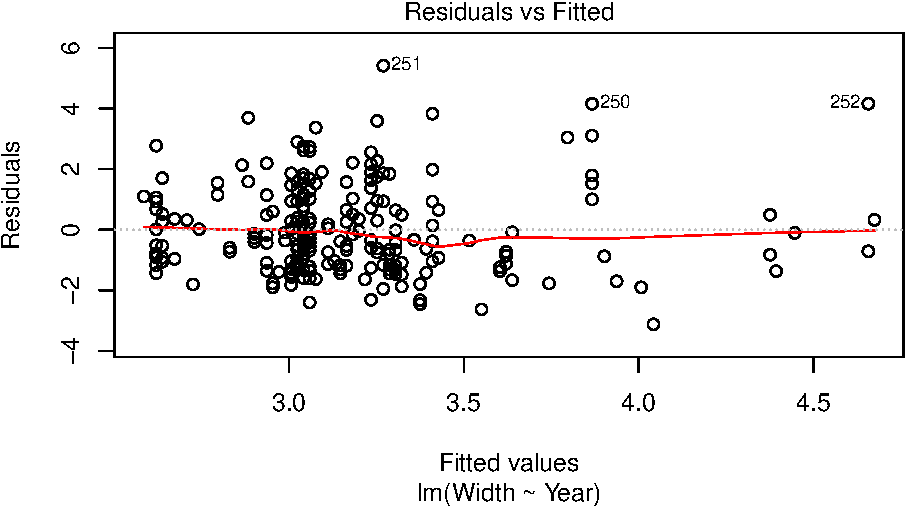
\includegraphics{02_Activity_AfterClass_files/figure-latex/unnamed-chunk-3-1.pdf}
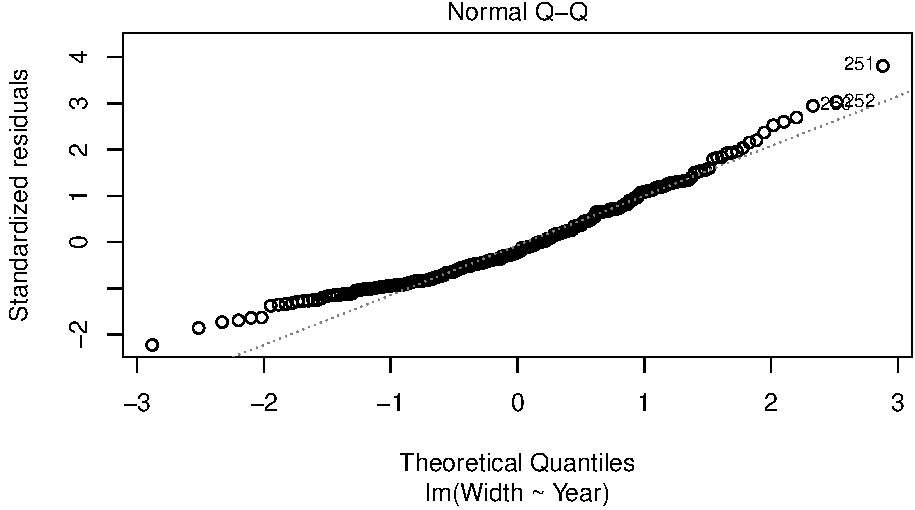
\includegraphics{02_Activity_AfterClass_files/figure-latex/unnamed-chunk-3-2.pdf}

This \textbf{first} plot illustrates a number of the key regression
assumptions, especially:

\begin{itemize}
\tightlist
\item
  Zero Mean
\item
  Linearity
\item
  Constant Variance
\item
  Normality (roughly)
\end{itemize}

We see that zero mean is met because the points are evenly distributed
above and below the horizontal line at 0 on the y-axis.

Linearity appears to be met since there is no persistent shape left to
the data.

Constant variance appears to be met in that there is not an apparent fan
shape where the model is doing a better job fitting the data at some
points (i.e., in older years) than at other points. We note that this
distribution isn't symmetric -- the y-axis points tends to be bound
between -2 and 4, which is what we saw in the histogram above; if it
were symmetric, it should be more evenly spread between, say, -2 and 2
or -4 and 4.

The \textbf{second} plot is another way of considering normality, other
than the histogram. A normal distribution would have all of the points
more or less on the diagonal line, since that would suggest a perfect
1-to-1 correspondence between the theoretical quantiles of a normal
distribution (x-axis) and the actual, standardized residuals on the
y-axis. Instead, curves in the bottom and top part of the line suggest
that the data are not normally distributed. For more details on
interpreting a QQ plot, see the OpenIntro textbook (especially p.95-99)
\href{https://drive.google.com/file/d/0B-DHaDEbiOGkRHNndUlBaHVmaGM/edit}{here.}

\end{document}
